%%%%%%%%%%%%%%%%%%%%%%%%%%%%%%%%%%%%%%%%%%%%%%%%%%%%%%%%%%%%%%%%%%%%
%% I, the copyright holder of this work, release this work into the
%% public domain. This applies worldwide. In some countries this may
%% not be legally possible; if so: I grant anyone the right to use
%% this work for any purpose, without any conditions, unless such
%% conditions are required by law.
%%%%%%%%%%%%%%%%%%%%%%%%%%%%%%%%%%%%%%%%%%%%%%%%%%%%%%%%%%%%%%%%%%%%

\documentclass[
  digital, %% The `digital` option enables the default options for the
           %% digital version of a document. Replace with `printed`
           %% to enable the default options for the printed version
           %% of a document.
%%  color,   %% Uncomment these lines (by removing the %% at the
%%           %% beginning) to use color in the digital version of your
%%           %% document
  notable,   %% The `table` option causes the coloring of tables.
           %% Replace with `notable` to restore plain LaTeX tables.
  twoside, %% The `twoside` option enables double-sided typesetting.
           %% Use at least 120 g/m² paper to prevent show-through.
           %% Replace with `oneside` to use one-sided typesetting;
           %% use only if you don’t have access to a double-sided
           %% printer, or if one-sided typesetting is a formal
           %% requirement at your faculty.
  nolof,     %% The `lof` option prints the List of Figures. Replace
           %% with `nolof` to hide the List of Figures.
  nolot,     %% The `lot` option prints the List of Tables. Replace
           %% with `nolot` to hide the List of Tables.
  %% More options are listed in the user guide at
  %% <http://mirrors.ctan.org/macros/latex/contrib/fithesis/guide/mu/fi.pdf>.
]{fithesis3}
%% The following section sets up the locales used in the thesis.
\usepackage[resetfonts]{cmap} %% We need to load the T2A font encoding
\usepackage[T1,T2A]{fontenc}  %% to use the Cyrillic fonts with Russian texts.
\usepackage[
  main=english, %% By using `czech` or `slovak` as the main locale
                %% instead of `english`, you can typeset the thesis
                %% in either Czech or Slovak, respectively.
  english, german, czech, slovak %% The additional keys allow
]{babel}        %% foreign texts to be typeset as follows:
%%
%%   \begin{otherlanguage}{german}  ... \end{otherlanguage}
%%   \begin{otherlanguage}{russian} ... \end{otherlanguage}
%%   \begin{otherlanguage}{czech}   ... \end{otherlanguage}
%%   \begin{otherlanguage}{slovak}  ... \end{otherlanguage}
%%
%% For non-Latin scripts, it may be necessary to load additional
%% fonts:
\usepackage{paratype}
\def\textrussian#1{{\usefont{T2A}{PTSerif-TLF}{m}{rm}#1}}
%%
%% The following section sets up the metadata of the thesis.
\thesissetup{
    date        = \the\year/\the\month/\the\day,
    university  = mu,
    faculty     = fi,
    type        = mgr,
    author      = Roman Oravec,
    gender      = m,
    advisor     = {Mgr. et Mgr. Jan Krhovják, Ph.D.},
    title       = {Modern obfuscation techniques},
    TeXtitle    = {Modern obfuscation techniques},
    keywords    = {keyword1, keyword2, ...},
    TeXkeywords = {keyword1, keyword2, \ldots},
    abstract    = {%
      This is the abstract of my thesis, which can

      span multiple paragraphs.
    },
    thanks      = {%
      These are the acknowledgements for my thesis, which can

      span multiple paragraphs.
    },
    bib         = example.bib,
    %% Uncomment the following line (by removing the %% at the
    %% beginning) and replace `assignment.pdf` with the filename
    %% of your scanned thesis assignment.
%%    assignment         = assignment.pdf,
}
%\bibliography{example.bib,references.bib}
\usepackage{makeidx}      %% The `makeidx` package contains
\makeindex                %% helper commands for index typesetting.
%% These additional packages are used within the document:
\usepackage{paralist} %% Compact list environments
\usepackage{amsmath}  %% Mathematics
\usepackage{amsthm}
\usepackage{amsfonts}
\usepackage{url}      %% Hyperlinks
\usepackage{markdown} %% Lightweight markup
\usepackage{tabularx} %% Tables
\usepackage{tabu}
\usepackage{booktabs}
\usepackage{listings} %% Source code highlighting
\usepackage{llvm/lang}  % include custom language for LLVM IR.
\usepackage{nasm/style} % include custom style for NASM assembly.
\lstset{
  basicstyle      = \ttfamily,
  identifierstyle = \color{black},
  keywordstyle    = \color{blue},
  keywordstyle    = {[2]\color{cyan}},
  keywordstyle    = {[3]\color{olive}},
  stringstyle     = \color{teal},
  commentstyle    = \itshape\color{magenta},
  breaklines      = true,
}
\usepackage{floatrow} %% Putting captions above tables
\floatsetup[table]{capposition=top}

\usepackage{minted} % Code highlighting
\setminted{
frame=lines,
framesep=2mm,
baselinestretch=1.2,
fontsize=\footnotesize,
linenos,
breaklines
}
\usemintedstyle{vs}
\usepackage{etoolbox,xpatch}

\makeatletter
\AtBeginEnvironment{minted}{\dontdofcolorbox}
\def\dontdofcolorbox{\renewcommand\fcolorbox[4][]{##4}}
\xpatchcmd{\inputminted}{\minted@fvset}{\minted@fvset\dontdofcolorbox}{}{}
\xpatchcmd{\mintinline}{\minted@fvset}{\minted@fvset\dontdofcolorbox}{}{} % see https://tex.stackexchange.com/a/401250/
\makeatother

\theoremstyle{definition}
\newtheorem{definition}{Definition}[section]

\begin{document}
\chapter{Introduction}
%\addcontentsline{toc}{chapter}{Introduction}

Intro goes here.

\chapter{Obfuscation}
 
This chapter describes some of the obfuscation techniques from a general point of view, as those principles can be applied to obfuscate a program on the source code, intermediate representation, or machine code level. The subsequent chapters will deal with implementation details for applying those methods to a program represented in the LLVM Intermediate Representation. 

\section{Obfuscating Transformations}

Collberg et. al \cite{taxonomy_obf} formally defines an \textit{obfuscating transformation} as follows:

\begin{definition}[Obfuscating transformation]{\ \\} \label{def:transformation}
Let $P \xrightarrow{\text{T}} P'$ be a transformation of a source program $P$ into a target program $P'$.
$P \xrightarrow{\text{T}} P'$ is an \textit{obfuscating transformation}, if $P$ and $P'$ have the same \textit{observable behavior}. More precisely, in order for $P \xrightarrow{\text{T}} P'$ to be a legal obfuscating transformation, the following conditions must hold:
\begin{itemize}
    \item If $P$ fails to to terminate or terminates with an error
condition, then $P'$ may or may not terminate.
    \item Otherwise, $P'$ must terminate and produce the same output as $P$. 
\end{itemize}
\end{definition}

This definition states that applying the transformations should preserve the input-output behavior of the program, but allows the obfuscated version of the program to produce some additional behavior, for example performing calls to the operating system or creating new files. 

The transformations may, and usually do, increase the computational complexity and memory requirements of the program. 

\subsection{Opaque predicates} \label{opaque}
Opaque predicates are common but effective constructs used for obfuscation. Constructing an opaque predicate consists of transforming a simple boolean expression into a complex one. 

\begin{definition}[Opaque predicate]
\label{def:opaque}
A predicate $P$ is opaque at point $p$ in a program, if its outcome is known at obfuscation time. We write $P_p^F (P_p^T)$ if $P$ always evaluates to \texttt{False} (\texttt{True}) at $p$, and $P_p^?$ if $P$ may sometimes evaluate to \texttt{True} and sometimes to \texttt{False} \cite{manufacturing_opaque}.
\end{definition}

Based on the possible values of an opaque predicate, we can distinguish two types:

\textbf{Invariant opaque predicates.} The value of the predicate is fixed, i.e. the obfuscator knows whether it evaluates to \texttt{True} or \texttt{False}, but its outcome is hard to deduce for the reverse engineer performing static analysis. 

\textbf{Two-way opaque predicates.} This type of predicates can evaluate either to \texttt{True} or \texttt{False} for all possible inputs. Collberg et al. \cite{taxonomy_obf} suggested using two-way opaque predicates as a branching point to two functionally identical branches, which can be created by cloning a single branch and applying different obfuscations on both of them. This makes the static analysis of the program harder while preserving the original functionality. 

Apart from types, opaque predicates can be categorized according to the methods of their construction: 

\textbf{Arithmetic-based opaque predicates.} They are constructed using hard-to-solve mathematical formulas and used to hide invariant properties of the predicate. The obfuscator uses a mathematical identity that always evaluates to the same boolean value. In Collberg's taxonomy \cite{taxonomy_obf}, this type of predicate falls into the \textit{trivial} category, because the deobfuscator can deduce its value by performing a static analysis restricted to a single basic block\footnote{Basic block is a sequence of instructions executed one-after-the-other with no branching\cite{dragonBook}} of a control flow graph. 

This kind of predicates is used in the \textit{Obfuscator-LLVM} in the \textit{Bogus Control Flow} pass, which adds a new basic block to the Control Flow Graph, but the branch leading to this new block is never taken. 

\textbf{Mixed Boolean-Arithmetic based opaque predicates.} This method is based on a technique described by Zhou et al. \cite{mba_zhou}, called \textit{Mixed Boolean Arithmetic} (MBA). 
MBA uses linear identities involving Boolean and arithmetic operations. MBA is further discussed in Section \ref{mba}.

\textbf{Alias-based opaque predicates.} This is one of the resilient methods proposed by Collberg et al. \cite{manufacturing_opaque} based on aliasing, i.e. state of a program where a particular memory location is referenced to by multiple pointers. When there is a possibility of aliasing, the static analysis might be much harder. In some cases, static alias analysis might be even undecidable \cite{aliasing_hard}.

Opaque predicates designed by Collberg et al. are constructed using two linked lists and two global pointers pointing into them. The opaque predicate then checks whether two pointers are aliasing, which always results in \texttt{False} since the two global pointers always refer to nodes within different lists. 

\textbf{Environment-based opaque predicates.}
This method uses system calls or library calls which guarantee that the result of a predicate using such calls will always be either \texttt{True} or \texttt{False}. 

An example of such opaque predicate is calling the \texttt{strcpy}\footnote{https://www.cplusplus.com/reference/cstring/strcpy/} function from the C standard library and comparing the returned value (pointer to the destination array) with the first argument supplied to the function.

\textbf{Bi-opaque predicates.} This method of constructing opaque predicates has been recently introduced by Xu et al. \cite{bi_opaque}. The advantage of bi-opaque predicates is that they are resilient against symbolic execution engines, such as Triton\footnote{https://triton.quarkslab.com/}, angr\footnote{https://angr.io/} and BAP\footnote{https://github.com/BinaryAnalysisPlatform/bap}. The tool\footnote{https://github.com/zzrcxb/fusor} developed by Xu et al. is built on \textit{Obfuscator-LLVM}, but replaces the trivial arithmetic-based opaque predicates with more resilient \textit{symbolic} opaque predicates, which exploit various weaknesses of symbolic execution. The \textit{bi-opaque} property means that these predicates can introduce \textit{false positives} to the analysis, which may make the reverse engineer falsely recognize legitimate predicates as opaque predicates.

Opaque predicates can be used to enhance other obfuscation methods, for example, the dead code insertion, described in \ref{dead}. 

\subsection{Instructions Substitution} \label{substitution}
Instructions substitution is one of the most simple obfuscation techniques. The principle of this method is to replace instructions containing binary arithmetic operations, such as addition and subtraction, and binary boolean operations, such as logical AND or XOR, with more complicated sequences of code, which yield the same result. 

Despite its simplicity, this technique is still used in current obfuscation tools. For example, \textit{Obfuscator-LLVM} uses simple substitutions using expressions composed exclusively of arithmetic operations to substitute addition and subtraction, and expressions composed of boolean operations to substitute boolean XOR, AND and OR. Below are some of the substitutions implemented in \textit{Obfuscator-LLVM}:

$$
    \begin{aligned}
    &x + y \rightarrow -(-x + (-y))\\
    &x - y \rightarrow x + (-y)\\
    %(b&c) j (bˆ c)
    &x \vee y \rightarrow (x \wedge y) \vee (x \oplus y)\\
    %(!b&c) j (b&!c)
    &x \oplus y \rightarrow (\neg x \wedge y ) \vee (x \wedge \neg y)\\ 
    \end{aligned}
$$

In contrast, \textit{Tigress} implements obfuscations that transform standard binary operators with more complex expressions in MBA (\ref{mba}) form. A list of such identities can be found in \cite{hackers_delight}, where the authors suggest using them to build efficient low-level operations for manipulating bit strings and numbers. Zhou et al. described a way to use such identities in \cite{mba_zhou}, while also showing that there is an unlimited number of them. 

This technique increases code diversification and it can be further improved by randomly choosing from several identities which can be used to substitute an instruction. 

It is also important to note that the compiler can optimize out this kind of transformation, therefore it should not be used for source-level obfuscation. It also implies that it should be run after the optimization passes if we are obfuscating at the intermediate representation level. 

A reverse engineer could use an optimizer on the obfuscated binary file to get rid of this transformation and reduce the complexity of the code for easier analysis. However, increased diversification of the code can still be useful, for example, to bypass an antivirus engine that is performing a static analysis of the program based on its signature, e.g. looking for known malicious patterns and sequences of instructions.

A rather bizarre example of this obfuscation technique is \textit{The M/o/Vfuscator}\footnote{https://github.com/xoreaxeaxeax/movfuscator}, created by Chris Domas. This is a tool inspired by the idea that the assembly instruction \texttt{mov} is \textit{Turing-complete}. It is able to compile a program written in C language into assembly code composed exclusively of \texttt{mov} instructions. The resulting Control-flow graph looks like a straight line and it would be probably very hard and time-consuming to reverse engineer. However, this obfuscator is more of a proof of concept than a practical tool, due to its impact on the performance of the compiled program. 

There is an even more extreme obfuscator worth mentioning, called \texttt{trapcc}\footnote{https://github.com/jbangert/trapcc}. It produces programs that are able to run without executing a single instruction of the CPU, leveraging Intel's Memory Management Unit fault handling mechanism. However, this is probably not considered an instructions substitution obfuscation in the true sense. 

\subsection{Garbage Code Insertion} \label{garbage}
This technique consists of inserting arbitrary instructions into the program without making an impact on the execution of the program. The total number of different programs possible
through garbage insertion is limited from above by the total number of free bits available for program space, which is limited only by available memory for program storage and is clearly enormous \cite{os_protection}. 

Similarly to instructions substitution, described in \ref{substitution}, the inserted code can be optimized out, therefore it should be applied after optimizing the program and it might get easily removed by a reverse engineer who is analyzing the program. 

This technique could be used to bypass simple automated malware analysis engines, as it breaks the signature of the program. The garbage instructions get executed, which adds complexity while performing dynamic analysis of the program, but on the other hand, it might impact the performance. 

A simple example of this technique is inserting \texttt{NOP} instruction into the assembly code. It does not have an impact on the program execution, but it's still reachable by the control flow of the program. A more advanced way to apply this method, described in \cite{os_protection}, is to insert spurious calls to the operating system, which could lead the attacker to analyze a large amount of garbage code and increase the time needed to perform the analysis. 

Yadegari et al. \cite{generic_deobfuscation} proposed a generic automated approach for deobfuscation of executable code based on taint analysis, which tracks the flow of values from the program's inputs to its outputs. This method can identify instructions that do not affect the execution of the program and remove the garbage instructions from the code. 

\subsection{Dead code insertion} \label{dead}
Dead code insertion is a technique similar to garbage code insertion, described in \ref{garbage}. The main difference is that the dead code adds a branch to the control flow of the program, but this branch is never taken during the execution of the program. 

This method was first introduced by Collberg et al. \cite{taxonomy_obf}. The paper suggests that there is a strong correlation between the perceived complexity of a piece of code and the number of predicates it contains. This technique could be further enhanced by using opaque predicates (\ref{opaque}) -- for example, adding a condition with an opaque predicate, which creates a branching point between a valid and a dead branch. The predicate would always evaluate to \texttt{True}, making it impossible for the control flow of the program to reach the redundant branch. 

Another way to further confuse the reverse engineer, described in \cite{taxonomy_obf}, is to add dummy blocks of code to the redundant branches. For example, one can clone a sequence of instructions from a valid block of code, introduce a bug into it and place it into the redundant (dead) branch. 

This transformation can be removed by utilizing optimization features including in modern compilers, as well as performing the automated deobfuscation approach proposed by Yadegari. et al. \cite{generic_deobfuscation}. An attack proposed by Salem and Bansescu \cite{ml_deobfuscation}, which is based on machine learning and pattern recognition algorithms to identify obfuscating transformations in the program, might also prove useful to a reverse engineer trying to remove this type of obfuscation. 

\subsection{Mixed Boolean-Arithmetic} \label{mba}
A mixed Boolean-arithmetic expression (MBA) is composed of integer arithmetic operations on n-bit words ($+,-,\times, \div$) and bitwise operations ($\wedge, \vee, \oplus, \neg$). Zhou et al. \cite{mba_zhou} present a method to generate an unlimited supply of MBA transforms based on MBA expressions, MBA identities and invertible functions, which can be used to obscure secret constants, intermediate values, and algorithms, while preserving original functionality. %TODO

The resulting MBA expressions are dependent on program input, so they can not be simplified by compiler optimization. 

There is a practical example in \cite{mba_zhou} of encoding a constant value $K=0x87654321$ as a multiterm polynomial MBA function $f(x_1,...,x_m) = K$ for arbitrary $x_1,...,x_m$.

The example uses a polynomial

$$ f(x) = 727318528x^2 + 3506639707x + 6132886 \pmod{2^{32}}$$

with $K$ as an input, which results in the value 1704256593. Since $f$ is an invertible function, $f^{-1}$ returns the original value of $K$. To make $f^{-1}$ dependent on the input of the program, the following linear MBA identity is combined with $f^1$:

$$2y = -2(x \vee(-y-1))-((-2x-1)\vee(-2y-1))-3$$

Note that the result of the right-hand side does not depend on the value of $x$, which can be an arbitrary integer from the program.  

To further obfuscate the MBA expression, another identity is applied:

$$x + y = (x\oplus y) - ((-2x-1)\vee(-2y-1))-1$$

The resulting encoding can be found in the appendix of \cite{mba_zhou}.

Guinet et al. presented a tool called \texttt{arybo} \cite{guinet_arybo}, which analyzes the operations performed by MBA expressions at the bit-level. The tool is able to significantly simplify MBA expressions, thus presenting a possibility to circumvent this type of obfuscation. 

\subsection{Control Flow Flattening} \label{flatten}

This transformation was first described by Wang et al. in \cite{wang2001protection}. The goal of this technique is to obscure targets of the branches between the basic blocks and thus to make the static analysis of a program more difficult. 

First, the basic blocks of the function are put on the same nesting level, preceded by a new block, usually referred to as the \textit{dispatcher}. The dispatcher contains code that works as a \texttt{switch} statement, used to determine which basic block is going to be executed next. In addition to the dispatcher, a routing variable also needs to be created. Each time one of the original basic blocks terminates its execution, the routing variable is updated and the flow of control is transferred back to the dispatcher, which forwards the control flow to the next basic block, in accordance with the value stored in the routing variable. 

The main issue with control flow flattening is finding a way to make the information about the dispatcher, the routing variable, and its updating, difficult to analyze. In its naive implementation, where the routing values are hardcoded during the obfuscation (as seen in Figure \ref{fig:flattening}), it's easy to analyze the code of the basic blocks and reconstruct the original control flow graph. 

In \cite{wang2001protection}, Wang et. al suggest use of global pointers, as in some cases, analysis of pointers can be proven to be NP-hard \cite{np_pointers}. In contrast, the authors of \cite{cappaert2010general} propose using one-way functions, which are always hard to analyze. 

Another issue with this obfuscation method is the computational overhead it introduces due to additional operations performed by the dispatcher. Johansson et. al \cite{johansson2017lightweight} proposed a novel method using lightweight dispatchers, which present a similar level of complexity for the reverse engineer as analyzing a flattened program augmented with cryptographic hash functions while reducing the overhead by one or more orders of magnitude.

\begin{figure}
    \begin{center}
        \begin{minipage}{.39\textwidth}
             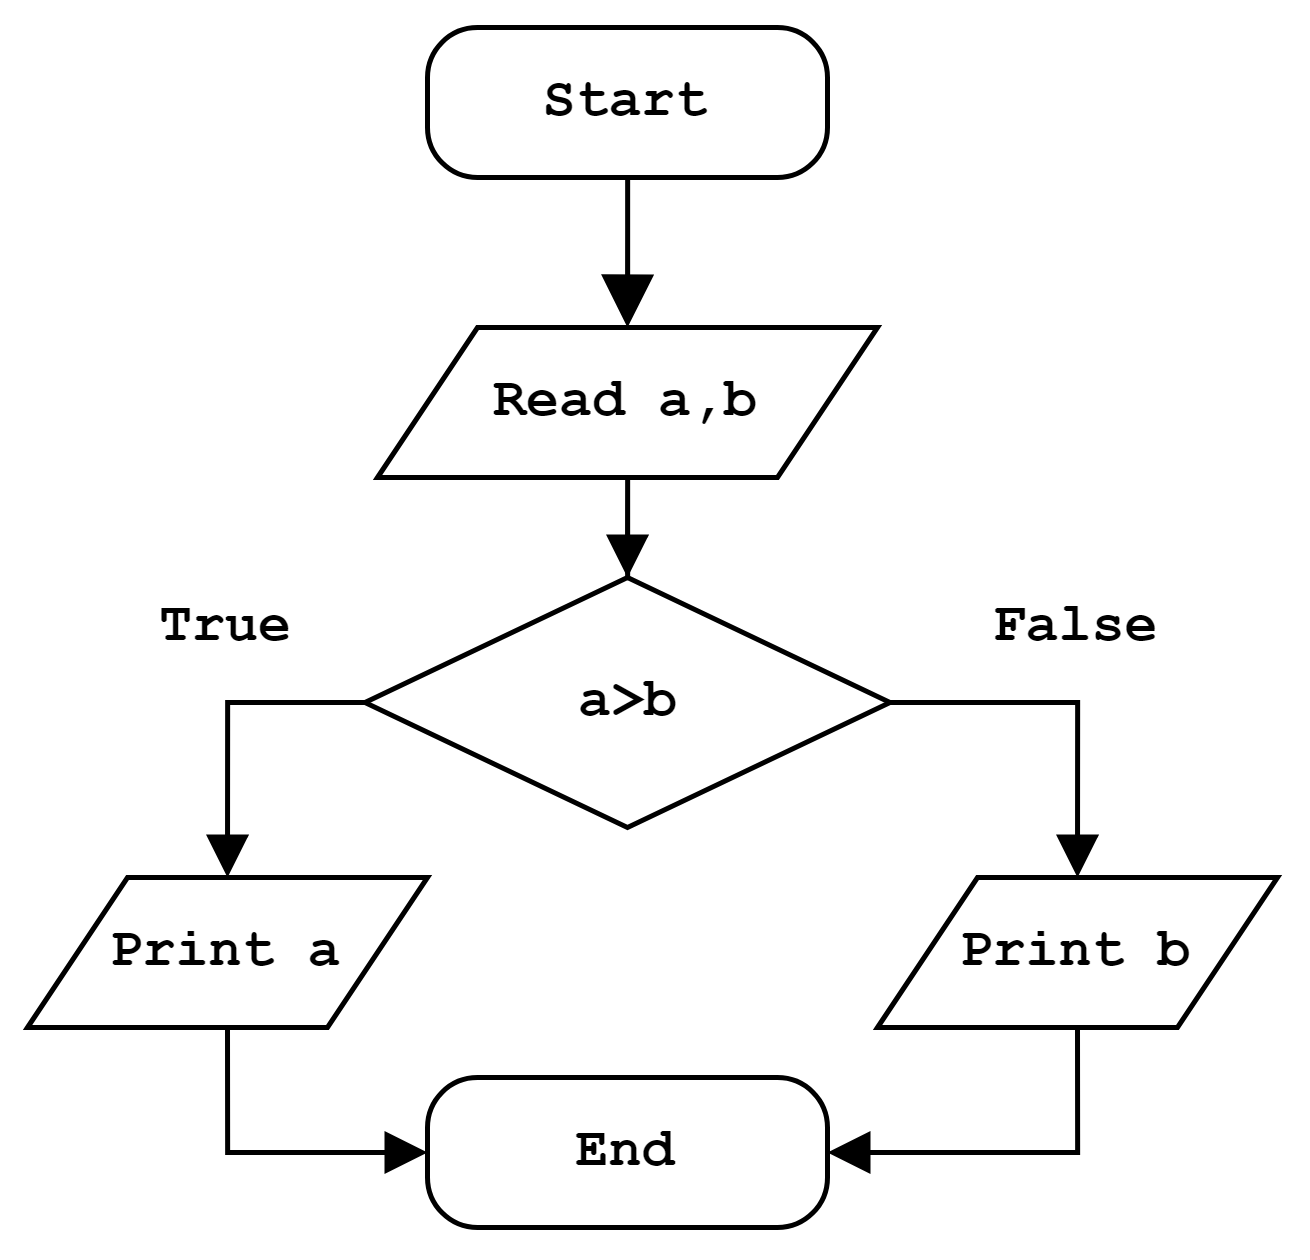
\includegraphics[width=\textwidth]{notflat.png}
        \end{minipage}
        \begin{minipage}{.6\textwidth}
             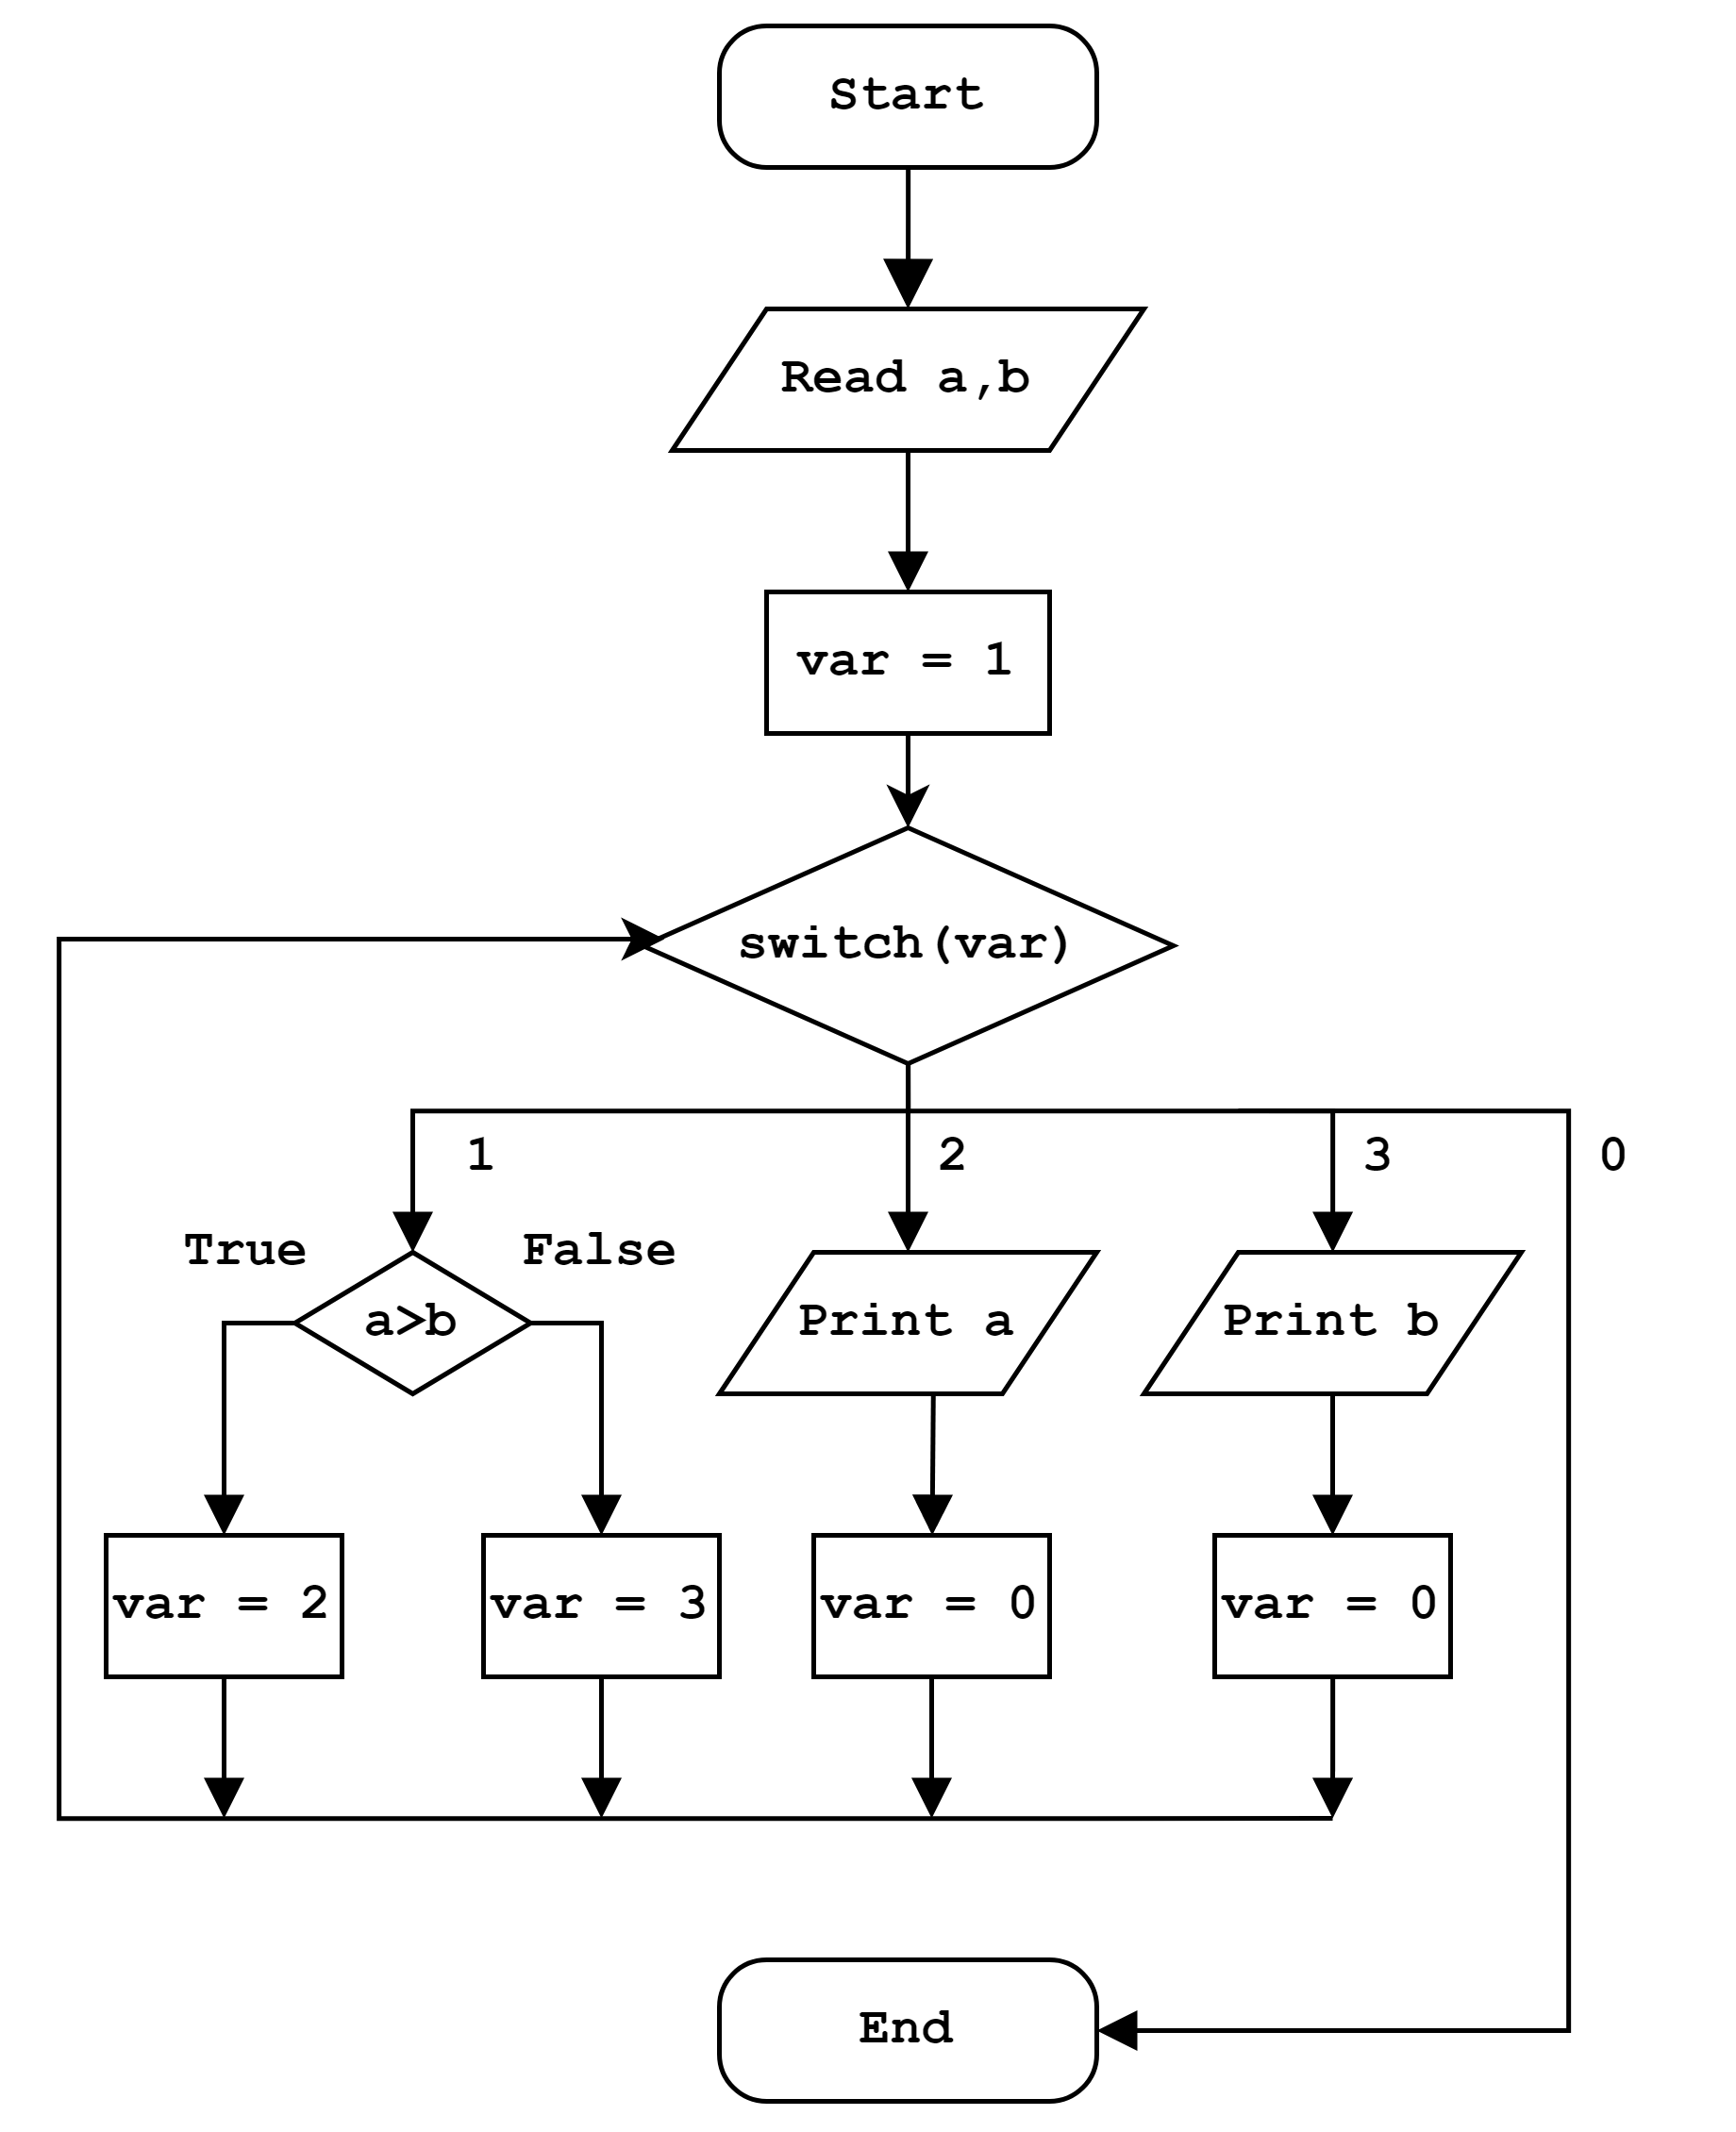
\includegraphics[width=\textwidth]{flat.png}
        \end{minipage}
    \end{center}
    \caption{Flowchart of a simple program returning a maximum of two numbers, before and after flattening. Notice that the comparison and print statements are on the same level of nesting after being flattened.}
    \label{fig:flattening}
\end{figure}

%TODO add more, maybe virtualization

\section{Evaluating Obfuscating Transformations} \label{sec:eval}
Determining usefulness of an obfuscating transformation is a complex task. When designing and evaluating an obfuscating transformation, one needs to consider multiple criteria, such as how hard would it be for an adversary (e.g. a reverse engineer) to understand the functionality of an obfuscated program $P'$, how hard would it be to construct a deobfuscator, or how much resources would a deobfuscator need to reconstruct the original program $P$, given $P'$ as an input. Unless the deobfuscation process is fully automated, these criteria will never be fully objective, since they will always, at least partly, depend on cognitive abilities of the attacker. 

Collberg et al. proposed some metrics \cite{taxonomy_obf}, which can be used to quantify and approximate the quality of obfuscation methods. They have defined the following three criteria: 
\begin{itemize}
    \item \textit{Potency} consists of various metrics which were originally designed to be used to measure software complexity in the field of software engineering, for example the number of operators and operands in $P$, number of predicates (cyclomatic complexity) in a function, or a nesting level of conditional statements in a function.
    
    \item \textit{Resilience} is measured on a four point scale, ranging from \textit{trivial} to \textit{one-way}. The value of resilience depends on two parameters -- \textit{programmer effort} -- how much time would a programmer need to construct a deobfuscator to reduce the \textit{potency} of a transformation, and \textit{deobfuscator effort} -- time and space complexity of a deobfuscator which can reduce the \textit{potency} of a transformation. \textit{Programmer effort} is based on the scope of the transformation, from local to inter-process, while \textit{deobfuscator effort} could be either polynomial or exponential.
    \item \textit{Cost} of a transformation measures how much execution time and space overhead would a transformation introduce to the obfuscated program. This value is also measured on a four point scale, ranging from \textit{free} (transformation adds a constant overhead) to \textit{dear} ($P'$ requires exponentially more resources than $P$).
\end{itemize}

Mohsen and Pinto \cite{eval2016} proposed using Kolmogorov complexity \cite{Kolmogorov1998} to measure the quality of obfuscation. Kolmogorov complexity can be described as the shortest length of a program, which can produce given object (e.g. a binary string, or an obfuscated program). Due to the undecidability of the halting problem, exact Kolmogorov complexity can not be computed. However, it can be estimated using compression algorithms. More specifically, Kolmogorov complexity is the lower bound of a compression algorithm.  

The idea to use Kolmogorov complexity to quantify the quality of obfuscation is based on an assumption that obfuscation produces irregularities in the obfuscated code (e.g. by inserting opaque predicates, or cloning diversifying basic blocks), thus making it less comprehensible for the adversary. A program that contains more regular patterns can be compressed with higher rate, and thus has a lower Kolmogorov complexity. In contrast, an obfuscated program would have higher Kolmogorov complexity, which implies that it is a usable metric for evaluating obfuscation, as shown in \cite{Kolmogorov1998}. 

\chapter{LLVM}

The LLVM Project started as a research project at the University of Illinois focused on creating a compiler framework designed to support transparent, life-long program analysis and transformation for arbitrary programs, by providing high-level information to compiler transformations at compile-time, link-time, run-time, and idle time between runs \cite{llvm_orig}. 

The name LLVM was originally an abbreviation for \textit{Low Level Virtual Machine}. Since the project has little in common with what is currently perceived as a virtual machine, the meaning of the abbreviation has been later removed to avoid confusion, so now LLVM is the full name of the project\footnote{\url{https://llvm.org/}}.

The project consists of various sub-projects, such as LLVM Core libraries providing source and target-independent optimizer and code generator, implementation of the C++ standard library with full support for C++11 and C++14, Clang -- a compiler for C, C++, and Objective-C, and the LLDB debugger.

\section{LLVM Compiler Architecture}
The LLVM compiler pipeline consists of three main phases. First, the frontend parses the input code, which includes validation of syntax and semantics and diagnosing errors. If the code is valid, the frontend creates a representation of the code in the LLVM Intermediate Representation (IR), which is discussed in further detail in the following section. 

Various analysis and transformation passes can be run on the IR. Analysis passes are used to gather some higher-order information about the IR without mutating it, e.g. generate the Control Flow Graph. Transformation passes mutate the IR in some way, for example deleting dead code. Transformation passes can use the results generated by the analysis passes. 

The part of a compiler that is responsible for these tasks is typically called the \textit{optimizer}. The main goal of the optimizer is to gather information about the runtime behavior of the program and apply it to improve the final code generated by the compiler. The most common goal of the optimizer is to make the program run faster. However, depending on the application, there can be other goals of optimization which would have higher priority. In the case of embedded systems, it could be reducing the size of the compiled code or analyzing the energy consumption of the program in order to make it more energy-efficient\cite{energy_consuption}. 

Lastly, the backend takes the IR as an input, performs passes like instruction selection and register allocation, and produces native machine code for the target architecture. This compiler pipeline is usually referred to as a \textit{three-phase compiler}.

\begin{figure}
    \centering
    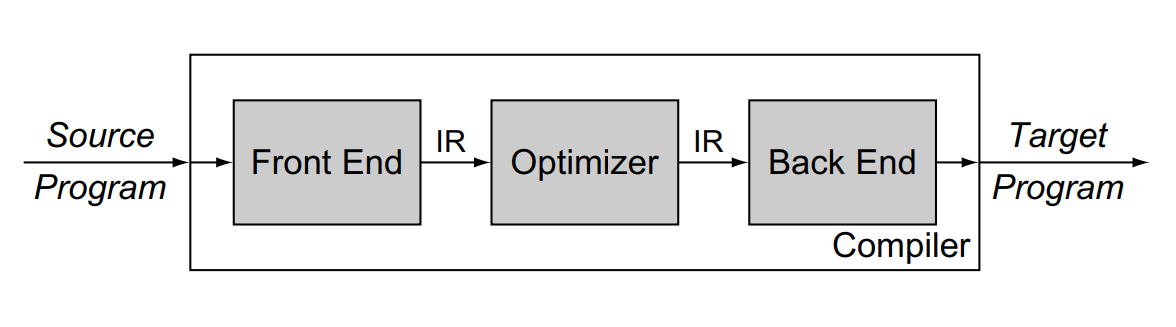
\includegraphics[width=\textwidth]{3phase.png}
    \caption{A high-level illustration of a three-phase compiler \cite{eng_comp}}
    \label{fig:3phase}
\end{figure}
    
The design of the LLVM compiler provides much flexibility, given that the IR is source and target-independent, therefore the optimization passes can be applied while compiling source code of any programming language which has an LLVM frontend. Some of the supported languages are C and C++, Go, Haskell, Rust, and Swift. 

LLVM backends, which generate the machine code from the intermediate representation, also support various target architectures, such as x86, ARM, and PowerPC.

For the purpose of obfuscation, the focus of this thesis is the middle section of the pipeline. Even though the optimizer works only with the intermediate representation form, which is passed to the backend afterward, transformations applied in this phase have an impact on the structure of the final executable file. 

\section{LLVM Intermediate Representation}
The LLVM IR is a low-level language similar to assembly. However, it provides various abstractions which remove target-specific instructions and features. It uses a set of infinite temporary registers and the \textit{Single Static Assignment} (SSA) form, which means that it needs to fulfill two constraints:

\begin{enumerate}
    \item Each definition has a distinct name,
    \item Each use refers to a single definition.
\end{enumerate}

 The  single-assignment  property  of  the  name  space  allows  the  com-piler to sidestep many issues related to the lifetimes of values; for example,because names are never redefined or killed, the value of a name is avail-able along any path that proceeds from that operation. These two properties simplify and improve many optimization techniques\cite{eng_comp}.

The Intermediate Representation is organized into modules -- each module corresponding to a single source file (also referred to as translation unit). During the compilation process, separate modules are linked with the LLVM Linker, also called LLD, to produce the executable file. Modules generally contain functions and global variables, both of which are called \textit{global values}. Global values are represented by a pointer to a memory location and their identifiers begin with the '@' character. In addition to global value identifiers, there are also local identifiers, prefixed with the '\%' character. They are typically used for register names and types. 

\begin{listing}
    \inputminted{llvm}{example.ll}
    \caption{Example of a short LLVM IR module. Some parts, such as target architecture information, metadata, and comments, have been omitted for better readability. Also, the compiler optimizations have been disabled.}
    \label{fig:ir_example}
\end{listing}

Figure \ref{fig:ir_example} shows a simple program in LLVM IR, which can be used to further introduce the LLVM IR syntax. On the first line, there is a definition of a global variable, a constant string, named \texttt{.str}. It consists of 12 characters, size of each of them is 8 bits. The \texttt{private} keyword states that this value is only directly accessible by objects in the current module and \texttt{unnamed\_addr} indicates that the address is not significant, only the content. Constants marked like this can be merged with other constants if they have the same initializer. 


The module defines two functions -- \texttt{foo} and \texttt{main} -- starting on lines 3 and 20 respectively. Every function definition starts with the \texttt{define} keyword and specifies the function's return type (a 32-bit integer in this case). The is also and external declaration of \texttt{puts} function, which is called in the \texttt{main} function to print the "Hello world" string. The main function then performs a call the \texttt{foo} function and terminates by returning zero. The \texttt{foo} function consists of multiple basic blocks. Every basic block is prefixed with its name and a colon and ends with a terminator instruction, such as \texttt{br} (branch) and \texttt{ret} (return). The function simply adds two integers (7 and 42), compares the result with another integer, and transfers the control flow to the next basic block, based on the result of the comparison. 

The SSA form, described at the beginning of this section, introduces a special type of instructions, called \texttt{phi} instructions. They appear at the point where different paths of control flow merge, as we can see at line 16 in Figure \ref{fig:ir_example}. The \texttt{phi} instruction assigns a value to the virtual register named \texttt{\%retval.0}, depending on the block from which the control entered the current block. If the control entered from the \texttt{\%if.then} block, value 7 is assigned. Otherwise, the control entered from the \texttt{\%if.end} block and the value stored in the virtual register \texttt{\%add} is chosen. 

The example code in Figure \ref{fig:ir_example} has been generated and tweaked to present a simple and readable form of the LLVM IR. First, \texttt{clang} was used to produce a human-readable form of the IR:

\begin{lstlisting}[language=bash]
$ clang -S -emit-llvm -c example.c -O0 -Xclang  
-disable-O0-optnone -fno-discard-value-names 
-o example.ll
\end{lstlisting}

The \texttt{-O0} flag tells \texttt{clang} to not perform any optimizations on the file. However, to be able to additionaly apply passes using \texttt{opt}, we need to include the \texttt{-Xclang -disable-O0-optnone} flags. Thanks to the \texttt{-fno-discard-value-names} flag, the IR contains meaningful names of the registers and basic blocks, instead of numbers only (e.g. \texttt{\%1, \%2}).

Then the \texttt{opt} tool is used to apply the \texttt{mem2reg} pass on the IR to transform it into a more simple form by promoting memory references into register references\footnote{\url{https://llvm.org/docs/Passes.html##mem2reg-promote-memory-to-register}}:

\begin{lstlisting}[language=bash]
$ opt -mem2reg -S example.ll -o example.ll
\end{lstlisting}

\chapter{Existing tools}

\section{Obfuscator-LLVM} \label{sec:ollvm}

Obfuscator-LLVM is an open-source project initiated in 2010. It aims to provide increased software security through code obfuscation and tamper-proofing\footnote{Preventing a user from modifying the software against the manufacturer's wishes.}. The project is a fork of the LLVM compilation suite, therefore it works with the LLVM IR, utilizing LLVM's possibility of writing custom transformation passes. It supports all programming languages and target platforms which are currently supported by LLVM. 

The open-source version of the project implements three obfuscating transformations:
\begin{enumerate}
    \item \textit{Instructions Substitution} is the most simple obfuscating transformation included in the project. It replaces simple binary operations with more complex ones, as described in Section \ref{substitution}. Obfuscator-LLVM supports substitution of integer additions and subtractions and the Boolean operators  AND  ($\&$),  OR  ($|$)  and  XOR  (ˆ). For example, the expression $a = b \wedge c$ is substituted as $a = (b \oplus \neg c) \wedge b$. Some of the operations have multiple substitution candidates, which are chosen randomly to increase code diversity. A full list of the implemented substitutions can be found in \cite{obfuscator-llvm}. The substitutions are rather simple and according to the authors, this transformation  can easily  be  circumvented  by  re-optimizing  the  generated  code.
    \item \textit{Bogus Control Flow} modifies the control flow graph by inserting a new basic block before an existing one. The new basic block ends with an opaque predicate (\ref{opaque}), which always evaluates to \texttt{True}, making a conditional jump to the original basic block. The original basic block is also cloned, randomly filled up with various junk instructions, and inserted to the \texttt{False} branch leading from the new basic block. This cloned block is never reached, because of the invariant opaque predicate. The weakness in the implementation of this transformation is that it uses just a single opaque predicate: $$(y < 10\, ||\, x \cdot (x - 1) \mod 2 == 0)$$ The two global variables, $x$ and $y$, which are declared to construct this predicate, can also give a hint on where the opaque predicates are, which would make it easier for a reverse engineer to overcome this transformation. 
    \item \textit{Control Flow Flattening} is implemented in a naive way, as described in Section \ref{flatten} -- by hardcoding the routing values during the obfuscation process. This implementation provides some resilience against automated analysis tools, e.g. signature-based malware scanners, but it does not propose a significant challenge for a reverse engineer or automated tools performing a more complex static analysis.
\end{enumerate}

Apart from the aforementioned obfuscating transformations, Obfuscator-LLVM also implements a transformation pass for basic block splitting. This pass introduces additional complexity to the transformations manipulating the control flow. 

The authors also added a feature to tag specific functions, which are supposed to be obfuscated, in the source code of the program. This way, the developers can reduce the negative performance impacts on the program they are obfuscating, by ommiting non-crucial functions from the obfuscation process. 

Commercial version of Obfuscator-LLVM used to implement additional, more advanced capabilities, such as code tamper-proofing and procedures merging, mentioned in \cite{obfuscator-llvm}. However, according to the wiki on the project github repository\footnote{\url{https://github.com/obfuscator-llvm/obfuscator/wiki}}, the commercial version is no longer available since the end of 2016. 

The github repository, containing the open-source version, is not being maintained since then as well. The authors of the project apparently founded a startup named Strong.Codes, which has been later acquired by Snap Inc.\footnote{\url{https://www.venturekick.ch/strongcodes}}.

\section{Tigress}

Tigress is a source-to-source obfuscator for C language, developed by Collberg\footnote{The co-author of \cite{taxonomy_obf}, \cite{manufacturing_opaque} and others} as a research project at the University of Arizona. Compared to Obfuscator-LLVM, while supporting only C language, Tigress seems to be a much more powerful obfuscation tool with a wide variety of implemented transformations, such as:
\begin{enumerate}
    \item \textit{Virtualization} turns a function into an interpreter with a custom set of virtual instructions for each function\footnote{\url{https://tigress.wtf/virtualize.html}}.
    \item \textit{Jitting (just-in-time compilation)} Turns the function to be obfuscated into a new one, which generates the machine code of the original function dynamically when it is executed. Another similar transformation supported by Tigress is \textit{JitDynamic}, which continuously modifies and updates the generated code at runtime. This version works at the granularity of basic blocks, decoding them when they need to be executed and subsequently re-encoding them.
    \item \textit{Flattening} implements a sligltly more advanced approach to flatten the control flow graph than the transformation implemented in Obfuscator-LLVM. Four kinds of block dispatchers are available -- basic implementation using \texttt{switch} statement, direct \texttt{goto} statements and indirect ones using a jump table, and \textit{call dispatch}, which creates a new function out of every basic block and uses a table of function pointers to jump to them. Obfuscation of the routing variable, which points to the next basic block to be executed, can be also enhanced by using opaque predicates (\ref{opaque}).
    
    %TODO
\end{enumerate}

\section{UPX (Ultimate Packer for eXecutables)}

\chapter{Design}

The core principle of building a new obfuscator is to use the foundations from Obfuscator-LLVM, while improving its currently available transformations and writing some new ones from scratch. Thanks to the modularity of the LLVM pass framework, each of the transformation passes can be applied independently, in a sequence, or together with the original Obfuscator-LLVM passes. 

Selected transformations are implemented with regard to their resilience against reverse engineering and impact on performance.

\section{Instructions substitution}
While applying basic rewrite rules for binary operations, such as the ones implemented in Obfuscator-LLVM, one can easily deobfuscate the expressions with an optimizing pass included in LLVM's \texttt{clang}, for example the \texttt{InstCombine}\footnote{\url{http://llvm.org/docs/Passes.html##instcombine-combine-redundant-instructions}} pass, which is supposed to "Combine instructions to form fewer, simple instructions." However, when the rewrite rules include MBA (\ref{mba}) expressions applied multiple times, the optimization fails to reconstruct the original expressions, as the experimental results in \cite{eyrollesMBAobf} imply. 

Based on the method for generating MBA identities proposed by Zhou et al. \cite{mba_zhou}, Eyrolles has generated a list of all rewrite rules composed of three boolean expressions \cite{eyrollesMBAobf}. We have decided to implement a selection of those rules in the obfuscator. For each binary operation, the rewrite rule is picked randomly out of three possibilities. to increase code complexity and diversity. Below are the rewrite rules implemented in the pass.

\subsection{Rewrite rules}
\subsubsection{Addition:}
$$
\begin{aligned}
%2*(x | y) - (x ^ y)
&x+y \rightarrow 2(x \vee y) - (x \oplus y) \\
%(x^(~y)) + 2*(x|y) + 1
&x+y \rightarrow(x \oplus \neg y)+ 2( x \vee y) + 1 \\
&x+y \rightarrow(x \oplus y)+2 y-2 (\neg x \wedge y) \\
\end{aligned}
$$

\subsubsection{Subtraction:}
$$
\begin{aligned}
%x - y --> 2*(x & ~y) - (x ^ y)
&x-y \rightarrow 2(x \wedge \neg y) - (x \oplus y) \\
% ~(~x + y) & ~(~x + y)
& x - y \rightarrow \neg ( \neg x + y) \wedge \neg(\neg x + y) \\
% x - y --> x & ~y - ~x & y
& x - y \rightarrow x \wedge \neg y - \neg x \wedge y \\
\end{aligned}
$$

\subsubsection{XOR:}
$$
\begin{aligned}
%x ^ y --> (x | y) - (x & y)
&x \oplus y \rightarrow (x \vee y) - (x \wedge y) \\
&x \oplus y \rightarrow(x \vee y)-y+(\neg x \wedge y) \\
&x \oplus y \rightarrow(x \vee y)-(\neg x \vee y)+(\neg x) \\
\end{aligned}
$$

\subsubsection{AND:}
$$
\begin{aligned}
%x & y --> (~x | y) - ~x
&x \wedge y \rightarrow (\neg x \vee y) - \neg x  \\
&x \wedge y \rightarrow(x \vee y)-(\neg x \wedge y)-(x \wedge \neg y) \\
&x \wedge y \rightarrow-(x \oplus y)+y+(x \wedge \neg y) \\
\end{aligned}
$$

\subsubsection{OR:}
$$
\begin{aligned}
&x \vee y \rightarrow(x \wedge \neg y) + y\\
&x \vee y \rightarrow(x \oplus y)+y-(\neg x \wedge y) \\
&x \vee y \rightarrow(x \oplus y)+(\neg x \vee y)-(\neg x) \\
\end{aligned}
$$

\section{Opaque constants} \label{obf_const}

To prevent the reverse engineer from extracting constant numerical values from the program, we have decided to implement a method proposed by Zhou and Main \cite{mba_zhou} to obscure the data by combining MBA identities (\ref{mba}) with invertible polynomials. 

Let:

\begin{itemize}
    \item $f$ be an invertible polynomial over $\mathbb{Z}/(2^n\mathbb{Z})$
    \item $g = f^{-1}$
    \item $E$ an MBA expression non-trivially equal to zero, for example $E = x + y - (x \vee y)-(\neg x \vee y)+(\neg x)$
    \item $C$ a constant to be obfuscated.
\end{itemize}

To obfuscate $C$, we can encode it as $C = g(E + f(C))$. The following example will show how the process works in practice. Suppose we are performing calculations in $\mathbb{Z}/(2^n)$ with 32-bit words\footnote{All calculations are $\mod 2^{32}$}, $f$ is a linear function with coefficient $a$ being an odd integer, so that it is invertible $\mod 2^{32}$ and $b$ is an arbitrary integer, while all integer values are 32 bits large:

\begin{align*}
C & = 123456 \\
a &= 1337 \\
b &= 42\\
x &= 1307300694 \\
y &= 2583472541 \\
f(x) &= ax + b = 1337x + 42\\
g(x) &= a^{-1}x + (-a^{-1}b) \\
&= 1337^{-1}x + (-1337^{-1}\cdot 42) 
\\&= 1185372425x + 1753965702 \\
E &= x + y - (x \vee y)-(\neg x \vee y)+(\neg x)
\end{align*}

Then we can encode $C$ as:

\begin{align*}
    f(C) &= 1337\cdot 123456 + 42 = 165060672 + 42 \\
    E &= 1307300694 + 2583472541 - 3724540895\\& - 3153898941 + 2987666601 = 0 \\
    C &= g(x + y - (x \vee y)-(\neg x \vee y)+(\neg x) + f(C)) \\
    &= g(0 + 165060672 + 42) \\
    &= 1185372425\cdot165060714 + 2541001594\\
    &= 123456 \mod 2^{32}
\end{align*}

The intermediate results of the functions $f$, $g$ and the MBA expression $E$ are calculated during runtime, which makes it much harder to obtain the value of $C$ during static analysis. The values of $a,b,x,y$ can be either randomly generated during compilation (obfuscation) time,  or by injecting a call to a random number generator which executes during runtime. The third option is to use suitable program inputs or function arguments, which would hinder deobfuscation techniques based on taint analysis\footnote{Tracking flow of values in the program and identifying values and variables that influence program's outputs, as well as the control flow of the program.}. 

For the purposes of testing and demonstration of this obfuscation method, we have chosen to generate the values of $a,b,x,y$ -- by using a random number generator during the compilation time.

\section{String obfuscation}

Strings, i.e. sequences of characters, are present in most of the existing programs. They are used to improve accessibility for the user interacting with the program, or to produce meaningful logging and error messages for the developers. For the reverse engineer, strings can present a valuable source of information about the program. They can be easily viewed in common decompiler and disassmbler software, as well as displayed in \texttt{bash} by using \texttt{strings}\footnote{\url{https://linux.die.net/man/1/strings}} command.

LLVM provides a convenient way to obfuscate all strings used in the program. During the obfuscation, the strings can be encoded using an arbitrary function which transforms them. Then, a decoding function is injected into the LLVM IR module. During runtime, the decoding function is used to obtain the original strings. This approach provides resilience against static analysis, while also introducing more complexity when performing dynamic analysis. 

The encoding and decoding functions can be different for each obfuscated program, which gives us a choice to either reduce the computational overhead by using an efficient and simple encoding and decoding function, or to strengthen the obfuscation by using more complex functions. When a keyed function is used, the key needs to be included in the obfuscated program. A possible way to harden this transformation is to use other obfuscation methods, such as the one mentioned in Section \ref{obf_const}, to hide the key.

\subsection{Encoding and decoding functions}
For the purposes of hiding the strings, we have used two simple functions, which can be used either individually, or combined. The first one shifts every character in the string by 13, e.g. it changes every character \textit{a}, represented in decimal as 97, to character \textit{n}, represented in decimal as 110.

The second, more complex function, uses a key, which is represented as a string. It iterates over the characters in the obfuscated string and performs a bitwise XOR, using a character on the corresponding position in the key string as a second operand. If the obfuscated string exceeds the length of the key, the function loops back to the first character of the key string. To add more confusion, this function obfuscates the string terminator (represented by decimal 0) as well.

\section{Bogus Control Flow} \label{des_bogus}

Bogus Control Flow pass is one of the passes included in \textit{Obfuscator-LLVM} (\ref{sec:ollvm}). The weakness of the original implementation is that it uses just a simple opaque predicate with two global variables, both initiated to zero. Any experienced reverse engineer could probably detect this type of opaque predicate by just simply looking at the disassembled program, while automated tools based on symbolic execution would definitely identify the predicate and simplify it. 

We have decided to improve this pass by replacing the weak opaque predicate by two types of stronger ones.

\subsection{Basic invariant opaque predicates}
Predicates of this type are composed of mathematical formulas which are always \texttt{True} (invariant). They include basic arithmetic operations ($+, -, \times, \div$) and remainder operations. MBA (\ref{mba}) is not used here, because running the Instructions Substitution pass would turn the simple operations into MBA anyways, therefore implementing them here as well would result in redundancy and decreased modularity. Following formulas, taken from \cite{loop}, are included in the pass:

$$
\begin{aligned}
x &\neq 7y^2 - 1  \\
0 &\neq (x^2 + 1) \mod7 \\
0 &\neq (x^2 + x + 7) \mod 81  \\
0 &\neq (4x^2 + 4) \mod 19 \\
\end{aligned}
$$

To further harden these predicates, we use input arguments of the obfuscated function for for the variables $x$ and $y$. Since the formulas are always true for an arbitrary integer, the predicate will always lead to a correct block. Using the function arguments in the opaque predicate may prevent various deobfuscation tools and techniques based on taint analysis (e. g. \cite{generic_deobfuscation}) from detecting and removing the predicate. 

When the function does not have suitable arguments, one or two global variables (depending on the number of available integer arguments) are created and initialized to a random value. 

\subsection{Symbolic memory opaque predicates} \label{sec:sym_mem}
This type of opaque predicate is based on the ideas first proposed by Collberg et al. \cite{manufacturing_opaque}. The exact method to construct is described in \cite{bi_opaque}. This is the technique which we have decided to implement\footnote{Although a similar implementation can be found at \url{https://github.com/hxuhack/symobfuscator}}. 

The predicate is constructed by creating two arrays and using an input value of the obfuscated function. The remainder $r$ after division of the input value by the size of the first array is used as an index to get the $r$=th element from the first array. This element then serves as an index to the second array, which yields an element from the second array that can be used to construct the opaque predicate. 

Since the value of the resulting element from the second array depends on the input symbol, detecting and removing this type of opaque predicate presents a hard problem (first described by King \cite{King1976}) for deobfuscation tools based on symbolic execution. 

\chapter{Implementation}
One way of integrating new passes using the LLVM framework is to include them in the LLVM source tree and build LLVM from source to use them during the compilation and obfuscation. The other way is to build an out-of-tree pass, which means to compile the source code of the pass separately, in an arbitrary destination, and load it with the LLVM \texttt{opt} tool to apply it on an LLVM IR module. We chose the out-of-tree method, as it is more convenient and straigtforward to use. 

To make the transformations more diverse, the passes use a random number generator based on the 64-bit Mersenne Twister by Matsumoto and Nishimura (\texttt{std::mt19937}), together with the \texttt{std::random\_device} interface to generate non-deterministic random numbers.
%TODO: general impl details
\section{Instructions substitution}
Implementation of this pass is based on a tutorial\footnote{\url{https://github.com/quarkslab/llvm-dev-meeting-tutorial-2015}} published by developers from Quarkslab, which shows how to write a simple obfuscating transformation which substitutes addition operation with an MBA expression. 
The pass iterates over instructions in a basic block, searching for instructions of \texttt{BinaryOperator} type that operate with integers. To build a new instruction, the \texttt{llvm::IRBuilder} class is used. 

For each substituted instruction, the pass generates a random number from a uniform integer distribution in range from 1 to 3 (number of available substitutions) using the random number generator described in the beginning of this chapter. After the new instructions are generated and their result is stored in a new virtual register, we call the \texttt{llvm::ReplaceInstWithValue()} function, which replaces all uses of the original instruction in the basic block, and removes the original instruction. 

This pass can be applied to the module multiple times, recursively generating more complex MBA expressions with each iteration. Listings 2 and 3 show how a simple instruction -- \texttt{\%add = add i32 \%a, \%b} -- which performs addition and stores the result in \texttt{\%add}, gets obfuscated after two iterations of this pass.

\begin{listing}
\begin{minted}{llvm}
  %2 = xor i32 %a, %b
  %3 = or i32 %a, %b
  %4 = mul i32 2, %3
  %add = sub i32 %4, %2  
\end{minted}
\label{lst:sub1}
\caption{IR code after using the substitution:\\ $x+y \rightarrow 2(x \vee y) - (x \oplus y)$.}
\end{listing}

\begin{listing}
\begin{minted}{llvm}
  %2 = xor i32 %a, -1
  %3 = xor i32 %a, -1
  %4 = or i32 %3, %b
  %5 = or i32 %a, %b
  %6 = sub i32 %5, %4
  %7 = add i32 %6, %2
  %8 = or i32 %a, %b
  %9 = mul i32 2, %8
  %10 = sub i32 0, %9
  %11 = add i32 %10, %7
  %12 = sub i32 0, %11
  %13 = sub i32 0, %9
  %14 = add i32 %13, %7
  %15 = sub i32 0, %14
  %add = and i32 %15, %12 
\end{minted}
\label{lst:sub2}
\caption{IR code from Listing 2 after substituting:\\
$x\oplus y \rightarrow(x \vee y)-(\neg x \vee y)+(\neg x)\\
x - y \rightarrow \neg ( \neg x + y) \wedge \neg(\neg x + y)$}
\end{listing}

\section{Opaque constants}
Boilerplate code for this pass is from Quarkslab developers blog\footnote{\url{https://blog.quarkslab.com/turning-regular-code-into-atrocities-with-llvm.html}}. However, the core principles and scope of obfuscation are fundamentally different. As described in Section \ref{obf_const}, this pass obfuscates unsigned 32-bit integer values. 

The main loop iterates over instructions of a basic block, ignoring those which are either a call to a function, switch, or a GEP\footnote{Get Element Pointer -- used to get the address of a subelement of an aggregate data structure.} instruction. When a suitable instruction is found, the pass checks whether some of its operands are constant 32-bit positive integers. Afterwards, the program proceeds to build an expression described in Section \ref{obf_const}. To find the modular inverse of $a$, \texttt{boost::integer::mod\_inverse()} function from the Boost\footnote{\url{https://www.boost.org/}} library is being used. Some of the values, most importantly, the multiplication of the obfuscated constant by the coefficient $a$ in function $f$, are computed during compilation time. Other parts, such as the expression $E$ and composition of functions $f$ and $g$, are created using the \texttt{llvm::IRBuilder}, which is instantiated with the first template argument being \texttt{NoFolder}. This template argument specifies a class used for constants. The default option -- \texttt{ConstantFolder} -- performs constant folding during compilation time, which could possibly weaken this obfuscating transformation, therefore \texttt{NoFolder} is used. 



\section{String obfuscation}
Implementation of this pass is partly based on a tutorial\footnote{\url{https://github.com/tsarpaul/llvm-string-obfuscator}} for building an LLVM pass for string obfuscation. The pass iterates over global variables in the IR file, since all strings in LLVM IR are stored as global variables. When a global variable that contains a string is encountered, it is encoded, so it does not appear in its original form in the resulting binary. 

Both encoding and decoding functions have to be provided in a separate LLVM IR module, named \texttt{codec.bc}. They have to be named \texttt{encode} and \texttt{decode} and their arguments need to be of type \texttt{unsigned char *}. 

For each encoded string, a call to a decoding function is created and inserted into the IR file. More specifically, a \texttt{decode\_stub()} function, which contains a call to a decoding function for every string, is injected at the beginning of the \texttt{main()} function in the obfuscated program. This approach has some disadvantages. At some point during the execution of the program, all of the strings will appear decoded. However, this transformation is still useful to hinder static analysis, as well as dynamic analysis, especially when the decoding function is obfuscated with other transformations. The second disadvantage is that the obfuscated program needs to have a \texttt{main()} function, otherwise the \texttt{decode\_stub()} function can not be injected. This second issue could possibly be solved by searching for other entry points of a program, apart from \texttt{main()}.

The main advantage of this pass is that the user can define arbitrary encoding and decoding functions (but also needs to ensure they are working correctly\footnote{Especially when obfuscating a program written in a language with different terminating characters than \texttt{'\textbackslash0}'.}). Both functions are first loaded from a separate LLVM module (*.bc file) using the \texttt{llvm::ParseIRFile()} function. Then, the functions can be stored in an object of \texttt{llvm::Function} type. While the \texttt{decode()} function is simply injected into the IR module, the \texttt{encode()} function is directly executed during the obfuscation, by utilizing the \texttt{llvm::ExecutionEngine} abstract interface.

To harden this obfuscation pass, we tell the compiler to always inline the decode function, by adding the \texttt{llvm::Attribute::AlwaysInline} attribute to it in the pass. This measure does not appear explicitly in the bitcode, since the inlining will be performed by the backend and the result is observable in the compiled program. 

\section{Bogus Control Flow}
The code for splitting and cloning the basic blocks is taken from the original Bogus Control Flow pass in \textit{Obfuscator-LLVM}, with just a slight modification. 

The original code had a bug in function \texttt{AddBogus()}, which is responsible for splitting the basic blocks, creating new branches and inserting placeholder instructions, which are later replaced by an opaque predicate. The bug is related to the exception handling mechanism in LLVM IR -- when a basic block might throw an exception, the terminator instruction at the end of the block is an \texttt{invoke} instruction, which can either lead to a regular basic block, or a special basic block that starts with a \texttt{landingpad} instruction and handles the thrown exception. The label of this block is marked with \texttt{unwind} keyword. 

However, when the block with \texttt{landingpad} is obfuscated, a new block, which starts with the opaque predicate, is inserted before the original one. This causes a situation when the \texttt{unwind} label leads to a block that does not start with \texttt{landingpad} instruction, generating an invalid IR module. Also, the new block with the \texttt{landingpad} instruction does not have an incoming edge marked as \texttt{unwind}, coming from an \texttt{invoke} instruction. Both of those facts result in a compilation failure.

Luckily, the \texttt{llvm::VerifierPass} was able to detect this erroneous behavior and display a corresponding error message. To fix this issue, we have added a check at the beggining of the \texttt{AddBogus()} function, to find out whether a block contains a \texttt{landingpad} instruction, so that such blocks can be skipped and not obfuscated. 

Our main contribution to this pass are the \texttt{getSimpleOP()} and \texttt{getSymOP()} functions, which construct the opaque predicates that are described in Section \ref{des_bogus}. First, the pass iterates through the obfuscated function arguments and stores those which are 32-bit integers. 

If such arguments are found, they are used to create an opaque predicate. In the \texttt{getSimpleOP()} function, the values of the obfuscated function arguments are divided by INT8\_MAX (127) and the remainders are used as the values for $x$ and $y$ in the formulas. This way, we prevent a situation when a result of some of the operations might overflow the type of the value where it is being stored, while we also reduce the computational overhead of the obfuscated program. One of the four formulas is then picked randomly to construct the predicate, which is inserted into the basic block afterwards. 

The implementation of the \texttt{getSymOP()} function is more complex. First, it allocates two arrays of integers on the stack and initializes their values (a range from 0 to array size minus one). Then, a remainder of a division of the input argument by the size of the first array is stored in a virtual register by creating a \texttt{srem} (signed remainder) instruction. This register is then used as the second index in a \texttt{getelementptr}\footnote{\url{https://llvm.org/docs/GetElementPtr.html}} instruction, indexing the first array. An element pointed to by the result of this \texttt{getelementptr} instruction is then stored into a new virtual register, which is used as an index for a second \texttt{getelementptr} instruction, indexing the second array. 

At this point, our implementation is a bit different from the design proposed in \cite{bi_opaque}. Since the values in the arrays correspond to the indices they are stored at, the elements obtained from both arrays are always equal. This allows us to construct an invariant opaque predicate by creating an \texttt{icmp} (integer comparison) instruction with the two elements as its operands, while the result of this comparison is always true. We suppose that this simplified implementation, however, does not weaken the resilience of the opaque predicates against symbolic execution, since we are still using the symbolic variable (input argument) to calculate the indices of the arrays.

Listing \ref{lst:sym} shows a snippet of the generated IR code that performs described operations (initialization of the arrays \texttt{\%arr1} and \texttt{\%arr2} is omitted). The obfuscated function is \texttt{main()} with standard arguments \texttt{(int argc, char *argv[])}, therefore the symbolic value used in this case is \texttt{\%argc}.

\begin{listing}[!h]
\begin{minted}{llvm}
%allocaInst = alloca i32
store i32 %argc, i32* %allocaInst
%loadInst = load i32, i32* %allocaInst
%load64 = sext i32 %loadInst to i64
%0 = srem i64 %load64, 8
%idx_1 = getelementptr inbounds [8 x i64], [8 x i64]* %arr1, i32 0, i64 %0
%1 = load i64, i64* %idx_1
%idx_2 = getelementptr inbounds [8 x i64], [8 x i64]* %arr2, i32 0, i64 %1
%2 = load i64, i64* %idx_2
%ArrOpq = icmp eq i64 %2, %1
\end{minted}
\caption{IR code for constructing symbolic opaque predicates.}
\label{lst:sym}
\end{listing}

\section{Limitations and possible extensions}
The passes have been implemented as a proof-of-concept for demonstration and testing purposes. Following ideas can be a topic for future research.
\begin{itemize}
    \item To make the obfuscation more user friendly, a scheduling pass can be implemented, which would run individual passes, together with LLVM optimisation passes, in a sequence specified by the user. 
    \item For deterministic results, a random number generator that could be seeded with a value provided by the user can be used instead of the current RNG. 
    \item For real-world projects, it would be useful to allow the user to annotate functions which are supposed to be obfuscated. Obfuscating only a selected subset of functions in a project would probably lead to smaller overhead from the obfuscation. 
\end{itemize}

\chapter{Testing and Evaluation}
In this chapter, we are to evaluate the obfuscation techniques based on the criteria and metrics described in Section \ref{sec:eval} 
and test the obfuscation on selected samples of code. The test programs consist of a C++ implementation of SHA-256 hash function\footnote{\url{https://github.com/martynafford/sha-2}}, a C++ implementation of AES-CBC\footnote{\url{https://github.com/kkAyataka/plusaes}} with 128-bit key, and an implementation of QuickSort in C\footnote{\url{https://www.programiz.com/dsa/quick-sort}}.

\section{Potency}
For testing potency, we are going to compute the software complexity metrics of the obfuscated bitcode, and compare it to the non-obfuscated version. 

Except for the Bogus Control Flow pass, the transformation do not significantly change the Control Flow Graph of the program, since the passes obfuscating constants and substituting instruction operate only in the scope of individual basic blocks, while the pass obfuscating strings manipulates global variables in the bitcode. It also injects a call to decode the string, but this operation does not change the CFG in a significant way. Therefore, we are going to use instruction count ($\mu_1$) and Kolmogorov complexity ($\mu_2$) as metrics to evaluate the potency of obfuscations. 

To obtain the values, we use \texttt{obfuscation-metrics} tool\footnote{\url{https://github.com/b-mueller/obfuscation-metrics}}, which includes an implementation of a simple LLVM analysis pass which parses the IR module and outputs the metrics. To compute Kolmogorov complexity, the tool uses the \texttt{llvm::zlib::compress()} function, which is included in the LLVM libraries. 

Table \ref{tab:changes} shows how applying the obfuscating transformations influence the complexity metrics, which allows us to estimate potency of the obfuscation. 

\subsection{Potency of individual passes}

The Instructions substitution pass has been applied on the test program in two iterations. Comparing the change of the metrics in the first and the second iteration, we can see that applying the transformation multiple times does increase $\mu_1$ more than $\mu_2$. This result implies that while the size of the program grows larger with each application of this pass, some regular patterns probably start to appear in the obfuscated program.

The results for the pass creating opaque constants show that it has relatively high potency. Character of the obfuscated programs might by a factor that contributes to this result. Even though we have used only one pair of functions to build the expressions for this obfuscation (as described in Section \ref{obf_const}), this pass inserts a large amount of new instructions (compared to the Instructions substitution pass), while also generating random operands for some of them, resulting in a significant increase of both metrics. 

String obfuscation comes out as the least potent transformation, but this result might be caused by the low number of strings in the obfuscated programs. Slightly higher potency in the case of using the string encoding and decoding functions based on bitwise XOR is caused by these functions being more complex, compared to the ones based on rotation of bits. 

Bogus Control Flow is the most potent pass, as it not only injects new instructions, but also duplicates the basic blocks and creates randomly initiated global variables. The significant increase of $\mu_1$ is probably caused by the creation of the symbolic memory opaque predicates (Section \ref{sec:sym_mem}), as it inserts an \texttt{alloca} instruction for each element of the arrays created in this process. On the other hand, metric $\mu_2$ might be mostly influenced by creation of randomized global variables, similarly as in the case of the Opaque constants transformation. 

\subsection{Combining the passes}

After evaluating each pass individually, we have determined the following sequence in which we apply all of the passes: \\

\textit{String obfuscation}\footnote{We have used the encoding and decoding functions based on bitwise XOR, since they have proved to have a higher potency.} $\rightarrow$ \textit{Bogus CF} $\rightarrow$ \textit{Opaque constants} $\rightarrow$ \textit{Substitution}. \\

The reasoning behind choosing this order of the passes is following: 

\begin{itemize}
    \item The String obfuscation pass injects new functions, which are not obfuscated, therefore it is reasonable to apply this pass first, so the subsequent passes can obscure these functions.
    \item Bogus Control Flow pass creates clones of the basic blocks, which would be easily identifiable without subsequent obfuscation. The opaque predicates are hardened and diversified by applying the substitution pass. 
    \item Expressions for hiding the constants also benefit from being applied before the substitution pass, same as the opaque predicates.
    \item Instructions substitution pass has basically the smallest scope -- transforming single instructions. Since it might improve the resilience and potency of all the other passes, it is applied last.
\end{itemize}

Table \ref{tab:changes} shows that combination of the passes results in significantly higher potency. We also present the values of $\mu_1$ and $\mu_2$ when the passes have been applied in a reverse order, where it is clearly visible how the particular ordering of the passes can influence the potency. In this case, the values are significantly lower than the original sequence. 

Due to the randomness of the obfuscation (e.g. randomly selecting the instruction substitution, randomly generating values for opaque constants), there is a slight variance in the resulting metrics when comparing obfuscated codes originating from the same program, after applying the same transformation independently. However, the variance was only around 4\%, therefore we do not include the results of multiple independent applications of the transformations in the table.

There is a noticeable pattern among all of the results in Table \ref{tab:changes}. Number of instructions ($\mu_1$) always increases more than Kolmogorov complexity ($mu_2$). This implies that the transformations have a larger influence on the size of the program, but they do not add irregularities to the program at the same rate. We suppose that this ratio can be more even, if add more diversity to the transformations, for example by implementing more substitution candidates for the instructions, creating arrays of various sizes for the symbolic memory opaque predicates, or by inserting random instructions into the cloned blocks in the Bogus Control Flow pass.

\begin{table}[!h] \label{tab:changes}
\begin{tabularx}{\textwidth} { 
  | m{10em} 
  | >{\centering\arraybackslash}X 
  | >{\centering\arraybackslash}X 
  | >{\centering\arraybackslash}X 
  | >{\centering\arraybackslash}X 
  | >{\centering\arraybackslash}X 
  | >{\centering\arraybackslash}X |}
\hline
Program  & \multicolumn{2}{c|}{SHA-512} & \multicolumn{2}{c|}{AES} & \multicolumn{2}{c|}{QuickSort} \\ \hline 
Metric & $\mu_1$ & $\mu_2$ & $\mu_1$ & $\mu_2$ & $\mu_1$ & $\mu_2$ \\ \hline \hline
Substitution & 1.37 & 1.07 & 1.09 & 1.04 & 1.23 & 1.03 \\ \hline
Substitution $\times2$  & 2.25 & 1.26 & 1.34 & 1.13 & 1.82 & 1.11 \\ \hline
Opaque constants        & 2.66 & 1.86 & 3.29 & 2.40 & 3.76 & 1.96 \\ \hline
String obfuscation 1    & 1.05 & 1.04 & 1.01 & 1.02 & 1.19 & 1.12 \\ \hline
String obfuscation 2    & 1.09 & 1.05 & 1.02 & 1.03 & 1.35 & 1.16 \\ \hline
Bogus Control Flow      & 3.52 & 2.23 & 4.28 & 3.49 & 7.18 & 3.40 \\ \hline
Str 2 + Bogus           & 3.72  & 2.35 & 4.40 & 3.64 & 10.64 & 4.44 \\ \hline
Str 2 + Bogus + Const   & 14.26 & 8.08 & 19.16 & 16.23 & 32.43 & 12.27 \\ \hline
All                     & 26.98 & 11.03 & 36.05 & 23.12 & 57.88 & 16.23 \\ \hline
Reverse order           & 8.10 & 4.24 & 9.50 & 7.05 & 21.57 & 7.84 \\ \hline
%  &         &         &           &  &  &  \\ \hline
\end{tabularx}
\caption{Changes in software complexity metrics after applying obfuscation. Values show a ratio of metrics of an obfuscated and a non-obfuscated program. $\mu_1$ is the change in the number of instructions, $\mu_2$ is the change of Kolmogorov complexity. Substitution $\times 2$ shows the effects of applying Instruction Substitution pass twice. String obfuscation 1 and 2 refer to the two different string encoding functions -- based on bit rotation and bitwise XOR, respectively. Last three rows show the changes of the metrics after applying multiple passes sequentially. Order of the passes in the \textit{All} row is String obfuscation 2 -- Bogus Control Flow -- Opaque constants -- Instructions substitution. In the last row, the values represent the metrics after applying this sequence in a reverse order. } 
\end{table}

\section{Resilience}

\section{Cost}

\chapter{Obfuscation of Android Native Code}

\chapter{Conclusion}


\printbibliography[heading=bibintoc] %% Print the bibliography.


\end{document}
